\documentclass{article}
\usepackage[paperwidth=487.254bp,paperheight=225.36bp,margin=0bp]{geometry}
\usepackage{anyfontsize}
\usepackage[scaled=1.0]{helvet}
\usepackage{tikz}
\usetikzlibrary{arrows.meta}
\renewcommand{\familydefault}{\sfdefault}
\pagestyle{empty}
\setlength{\parindent}{0pt}

\begin{document}
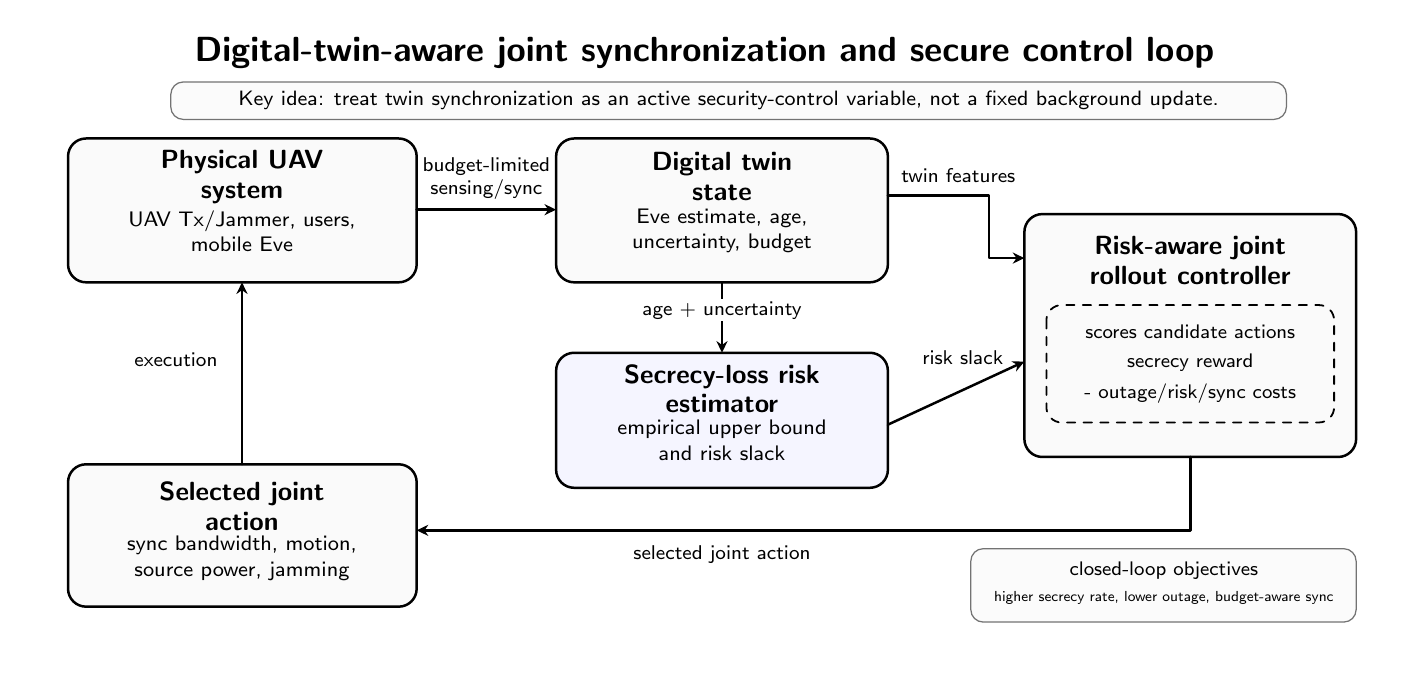
\begin{tikzpicture}[
  x=0.2642375bp,
  y=-0.26419695bp,
  line cap=round,
  line join=round,
  >={Stealth[length=4.2,width=4]},
  module/.style={draw=black, line width=0.9, rounded corners=6.5, fill=gray!4},
  smallbox/.style={draw=black!55, line width=0.45, rounded corners=4.5, fill=gray!3},
  arrow/.style={draw=black, line width=0.9, -{Stealth[length=4.2,width=4]}},
  label/.style={font=\sffamily\fontsize{7.2}{8.3}\selectfont, fill=white, inner sep=0.8},
  every node/.style={font=\sffamily, inner sep=0}
]
\path[use as bounding box] (0,0) rectangle (1844,853);
\fill[white] (0,0) rectangle (1844,853);

% Title and top note
\node[font=\sffamily\bfseries\fontsize{12.6}{14}\selectfont] at (922,34)
  {Digital-twin-aware joint synchronization and secure control loop};
\draw[smallbox] (195,74) rectangle (1715,125);
\node[font=\sffamily\fontsize{7.5}{8.5}\selectfont] at (955,99)
  {Key idea: treat twin synchronization as an active security-control variable, not a fixed background update.};

% Main modules
\draw[module] (55,151) rectangle (530,347);
\node[align=center, font=\sffamily\bfseries\fontsize{9.5}{10.7}\selectfont] at (292,203)
  {Physical UAV\\system};
\node[align=center, font=\sffamily\fontsize{7.6}{9.2}\selectfont] at (292,277)
  {UAV Tx/Jammer, users,\\mobile Eve};

\draw[module] (720,151) rectangle (1172,347);
\node[align=center, font=\sffamily\bfseries\fontsize{9.5}{10.7}\selectfont] at (946,203)
  {Digital twin\\state};
\node[align=center, font=\sffamily\fontsize{7.6}{9.2}\selectfont] at (946,277)
  {Eve estimate, age,\\uncertainty, budget};

\draw[module, fill=blue!4] (720,443) rectangle (1172,627);
\node[align=center, font=\sffamily\bfseries\fontsize{9.5}{10.7}\selectfont] at (946,492)
  {Secrecy-loss risk\\estimator};
\node[align=center, font=\sffamily\fontsize{7.6}{9.2}\selectfont] at (946,562)
  {empirical upper bound\\and risk slack};

\draw[module] (1358,254) rectangle (1810,585);
\node[align=center, font=\sffamily\bfseries\fontsize{9.5}{10.7}\selectfont] at (1584,317)
  {Risk-aware joint\\rollout controller};
\draw[dashed, line width=0.65, rounded corners=5.5] (1388,378) rectangle (1780,538);
\node[font=\sffamily\fontsize{7.1}{8.2}\selectfont] at (1584,414) {scores candidate actions};
\node[font=\sffamily\fontsize{7.1}{8.2}\selectfont] at (1584,456) {secrecy reward};
\node[font=\sffamily\fontsize{7.1}{8.2}\selectfont] at (1584,498) {- outage/risk/sync costs};

\draw[module] (55,595) rectangle (530,789);
\node[align=center, font=\sffamily\bfseries\fontsize{9.5}{10.7}\selectfont] at (292,652)
  {Selected joint\\action};
\node[align=center, font=\sffamily\fontsize{7.6}{9.2}\selectfont] at (292,723)
  {sync bandwidth, motion,\\source power, jamming};

\draw[smallbox] (1285,710) rectangle (1810,810);
\node[font=\sffamily\fontsize{7.1}{8.2}\selectfont] at (1548,740) {closed-loop objectives};
\node[font=\sffamily\fontsize{5.25}{6.1}\selectfont] at (1548,777)
  {higher secrecy rate, lower outage, budget-aware sync};

% Connections and labels
\draw[arrow] (530,248) -- (720,248);
\node[label, align=center] at (625,205) {budget-limited\\sensing/sync};

\draw[arrow] (946,347) -- (946,443);
\node[label] at (946,385) {age + uncertainty};

\draw[arrow] (1172,229) -- (1310,229) -- (1310,314) -- (1358,314);
\node[label] at (1268,202) {twin features};

\draw[arrow] (1172,541) -- (1358,455);
\node[label] at (1274,450) {risk slack};

\draw[arrow] (1584,585) -- (1584,685) -- (530,685);
\node[label] at (946,718) {selected joint action};

\draw[arrow] (292,595) -- (292,347);
\node[label] at (202,453) {execution};

\end{tikzpicture}
\end{document}
